\documentclass{article}

% ICLR 2027's style archive is not yet present in the official template repo.
% This draft uses the immediately preceding official style as a temporary shell.
\usepackage{template/iclr2026_conference,times}
\input{template/math_commands.tex}
\usepackage{hyperref}
\usepackage{url}
\usepackage{booktabs}
\usepackage{graphicx}
\usepackage{subcaption}
\usepackage{xcolor}
\usepackage{microtype}

\newcommand{\method}{\textsc{SpecKV}}
\newcommand{\todo}[1]{\textcolor{red}{[TODO: #1]}}

\title{Keys Decide, Values Describe: Acceptance-Aware KV Cache Compression for Speculative Decoding}

\author{Anonymous authors}

\begin{document}

\maketitle

\begin{abstract}
Speculative decoding accelerates language-model inference by asking a small draft
model to propose tokens for verification by a larger target model, but standard
implementations retain a separate key--value (KV) cache for each model. We study
how the draft cache can be compressed while preserving the quantity that directly
controls speculative speed: token acceptance. Our central observation is that
acceptance is strongly asymmetric in key and value precision. On a Qwen2.5-3B
target with a Qwen2.5-1.5B draft at 4K context, 8-bit keys and 4-bit values reduce
total target-plus-draft KV memory by 27.0\% while retaining 95.4\% of native
acceptance (0.544 versus 0.571). Reversing the assignment gives the same memory
saving but retains only 79.6\% of acceptance (0.454). Controlled Gaussian
perturbations expose the same mechanism: key noise changes attention routing and
rapidly destroys top-1 stability, whereas value noise is tolerated at much larger
magnitudes. Based on this observation, \method profiles each draft layer and cache
component under the actual speculative loop, then selects mixed precision under an
acceptance-drop budget. Exact full-precision target verification preserves the
target output distribution. We evaluate the hypothesis across Qwen2.5, Qwen3,
Llama 3, OLMo 2, and SmolLM2 model pairs and across 1K--4K contexts.
\end{abstract}

\section{Introduction}

Speculative decoding converts several serial target-model decoding steps into a
single parallel verification step by sampling proposals from a cheaper draft
model~\citep{leviathan2023speculative,chen2023speculative}. The method is
distribution preserving, but its systems footprint includes two model states and
two growing KV caches. This duplication becomes consequential at long context,
where each generated token reads the prefix cache and cache capacity limits the
number of concurrently served requests.

Quantizing the draft cache seems straightforward, but generic model-quality
metrics do not reveal whether a compressed cache remains a useful speculator. A
small distributional error can move the draft's top proposal away from the
target's token and terminate an entire speculative block. Conversely, errors in
directions irrelevant to the verifier may have little effect on acceptance. This
motivates an acceptance-aware rather than reconstruction-aware objective.

Our investigation starts from the attention decomposition
\begin{equation}
  A_\ell = \operatorname{softmax}\!\left(\frac{Q_\ell K_\ell^\top}{\sqrt{d_h}} + M\right),
  \qquad O_\ell = A_\ell V_\ell W_{O,\ell}.
  \label{eq:attention}
\end{equation}
Keys determine the routing distribution $A_\ell$, whereas values determine the
payload read after routing. We hypothesize that coarse key quantization is more
likely to redirect attention and cascade through subsequent layers than an
equal-memory reduction in value precision. This role asymmetry is compatible with
prior KV quantization analyses~\citep{liu2024kivi,hariri2025more}, but we ask a
different operational question: \emph{which errors can a draft model tolerate
without losing speculative acceptance?}

Our preliminary findings support three claims. First, Gaussian key perturbations
are dramatically more destructive to next-token stability than value
perturbations. Second, K8V4 consistently dominates K4V8 on Qwen2.5 despite their
identical memory cost. Third, a conservative layer-wise allocator can reduce the
draft cache while holding acceptance close to the full-precision draft. The
ongoing cross-family campaign tests whether this acceptance asymmetry generalizes
across architecture, scale, and context length.

\section{Background and Problem Formulation}

Let $p(\cdot\mid x_{\le t})$ be the target distribution and
$q(\cdot\mid x_{\le t};\widehat{\mathcal C}_d)$ the draft distribution produced
from a compressed draft cache $\widehat{\mathcal C}_d$. Standard speculative
sampling accepts proposals using the target correction rule; greedy speculative
decoding accepts the longest proposal prefix matching target argmax tokens. In
both cases, target verification makes the final sequence exact with respect to
the chosen target decoding rule. Compression affects efficiency through
acceptance, not final correctness.

For target and draft cache sizes $M_t$ and $M_d$, native speculative decoding uses
$M_t+M_d$. If layer $\ell$ stores keys and values with precisions
$b^K_\ell,b^V_\ell$, the compressed draft cost is approximately
\begin{equation}
  \widehat M_d \propto T \sum_{\ell=1}^{L_d}
  H^{KV}_\ell d_{h,\ell}\left(b^K_\ell+b^V_\ell\right),
\end{equation}
plus one scale per token and KV head in our per-vector quantizer. Total saving is
$(M_d-\widehat M_d)/(M_t+M_d)$; it is necessarily smaller than the percentage
saved from the draft cache alone.

\section{Method}

\subsection{Draft-cache fake quantization}

For a key or value vector $x$, we use symmetric per-vector fake quantization,
\begin{equation}
  s(x,b)=\frac{\max_i|x_i|}{2^{b-1}-1}, \qquad
  \widehat x=s\,\operatorname{clip}\!\left(\operatorname{round}(x/s),
  -2^{b-1}+1,2^{b-1}-1\right).
\end{equation}
Only the draft KV state is quantized between cached decode steps. The target model
and verifier remain in BF16. This simulator measures the algorithmic
memory--acceptance tradeoff without conflating it with a particular packed-cache
kernel.

\subsection{Acceptance-aware sensitivity profiles}

We first evaluate a full-precision draft baseline. Then, for each selected layer
$\ell$, component $c\in\{K,V\}$, and candidate bit width $b\in\{4,8\}$, we
quantize only $(\ell,c)$ while leaving all other draft-cache entries in BF16. The
measured risk is
\begin{equation}
  r_{\ell,c,b}=\max\left(0,\alpha_{\mathrm{BF16}}-alpha_{\ell,c,b}\right),
\end{equation}
where $\alpha$ is the end-to-end speculative acceptance rate. We additionally log
accepted tokens per verification round, top-1 match, acceptance mass,
Jensen--Shannon divergence, and exact agreement with greedy target decoding.

\subsection{Budgeted mixed-precision allocation}

Given one-at-a-time risks, our transparent initial allocator solves an additive
surrogate:
\begin{equation}
  \min_{\{b^c_\ell\}} \widehat M_d
  \quad \text{s.t.}\quad
  \sum_{\ell,c} r_{\ell,c,b^c_\ell}\leq\epsilon,
  \qquad b^c_\ell\in\{4,8,16\}.
  \label{eq:allocation}
\end{equation}
The additive approximation is deliberately conservative and is validated by
running the selected allocation through the complete speculative loop. A stronger
version will model cross-layer interactions rather than assuming independent
risks.

\section{Experimental Setup}

Our preliminary experiment uses Qwen2.5-3B as target and Qwen2.5-1.5B as
draft~\citep{yang2024qwen25}. We evaluate contiguous WikiText-2 validation blocks,
four draft proposals per verification round, greedy target verification, and 16
generated tokens per prompt. The 1K experiment uses 64 prompts; the 4K experiment
uses 16 prompts. The ongoing cross-family campaign uses the pairs in
Table~\ref{tab:model-pairs}. All target and draft pairs were checked for tokenizer
compatibility before launch.

\begin{table}[t]
  \caption{Cross-family campaign. Each pair is evaluated at 1K and 4K context,
  followed by top-eight-layer K/V sensitivity profiling and an acceptance-budgeted
  allocation.}
  \label{tab:model-pairs}
  \centering
  \small
  \begin{tabular}{lll}
    \toprule
    Family & Target & Draft \\
    \midrule
    Qwen2.5 & 3B, 7B & 1.5B, 3B \\
    Qwen3 & 8B & 4B \\
    Llama 3 & Llama-3.1-8B & Llama-3.2-3B \\
    OLMo 2 & 7B & 1B \\
    SmolLM2 & 1.7B & 360M \\
    \bottomrule
  \end{tabular}
\end{table}

We report acceptance rate, accepted tokens per target verification, top-1 match,
JS divergence, acceptance mass, draft-cache bytes, and total target-plus-draft KV
bytes. Python fake quantization does not provide a valid kernel-level speed
measurement, so we do not make throughput claims from this implementation.

\section{Preliminary Results}

\subsection{Keys are the fragile routing state}

Figure~\ref{fig:gaussian} perturbs all draft-cache keys or values with Gaussian
noise scaled to the clean activation standard deviation. At $\alpha=0.03$, key
noise reduces top-1 agreement with the clean draft to 0.617 and raises JS
divergence to 0.176. Value noise at the same magnitude retains 0.992 top-1 match
with JS divergence 0.0004. At $\alpha=0.1$, the corresponding top-1 matches are
0.109 for K and 0.953 for V. This large separation is consistent with routing
errors in $K$ changing $A$ in Equation~\ref{eq:attention} before values are read.

\begin{figure}[t]
  \centering
  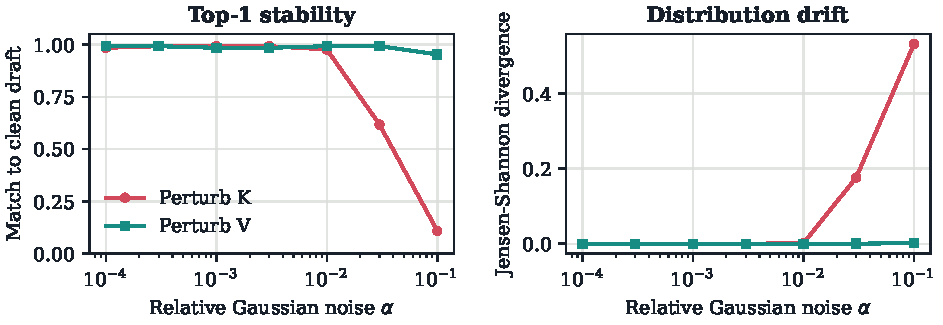
\includegraphics[width=\linewidth]{figures/gaussian_kv_sensitivity.pdf}
  \caption{Controlled perturbations of the Qwen2.5-1.5B draft cache. Keys are far
  more sensitive than values under both top-1 stability and distribution drift.}
  \label{fig:gaussian}
\end{figure}

\subsection{Equal memory does not imply equal acceptance}

Figure~\ref{fig:equal-memory} isolates the core comparison. K8V4 and K4V8 have
identical average precision and save the same KV bytes. At 1K context, K8V4 yields
0.475 acceptance versus 0.292 for K4V8. At 4K, the rates are 0.544 and 0.454,
respectively. The 4K K8V4 configuration retains 95.4\% of native acceptance while
saving 61.7\% of draft KV memory and 27.0\% of combined target-plus-draft KV
memory.

\begin{figure}[t]
  \centering
  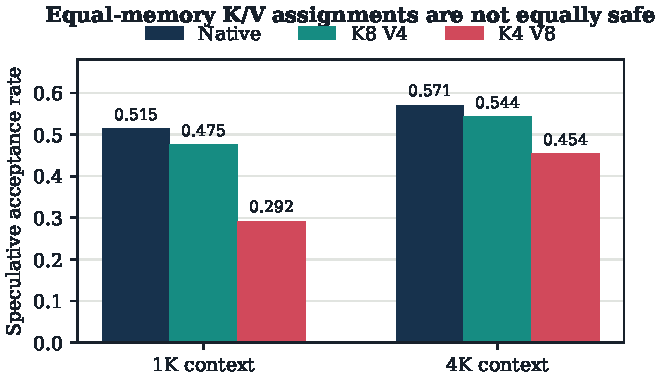
\includegraphics[width=0.78\linewidth]{figures/equal_memory_asymmetry.pdf}
  \caption{Speculative acceptance for two equal-memory asymmetric assignments.
  Preserving key precision consistently dominates preserving value precision.}
  \label{fig:equal-memory}
\end{figure}

\begin{table*}[t]
  \caption{Preliminary Qwen2.5-3B/1.5B results. ``Retained'' normalizes acceptance
  by the full-precision draft at the same context. Memory includes 16-bit scale
  metadata for each quantized KV vector.}
  \label{tab:preliminary}
  \centering
  \small
  \begin{tabular}{llrrrrr}
\toprule
Context & Draft KV & Accept. & Retained (\%) & Draft saved (\%) & Total saved (\%) & JS $\downarrow$ \\
\midrule
1K & FP16 & 0.515 & 100.0 & 0.0 & 0.0 & 0.071 \\
1K & K8 V8 & 0.495 & 96.1 & 49.2 & 21.5 & 0.086 \\
1K & K8 V4 & 0.475 & 92.4 & 61.7 & 27.0 & 0.088 \\
1K & K4 V8 & 0.292 & 56.7 & 61.7 & 27.0 & 0.189 \\
1K & K4 V4 & 0.300 & 58.3 & 74.2 & 32.5 & 0.189 \\
\midrule
4K & FP16 & 0.571 & 100.0 & 0.0 & 0.0 & 0.051 \\
4K & K8 V8 & 0.552 & 96.8 & 49.2 & 21.5 & 0.068 \\
4K & K8 V4 & 0.544 & 95.4 & 61.7 & 27.0 & 0.069 \\
4K & K4 V8 & 0.454 & 79.6 & 61.7 & 27.0 & 0.142 \\
4K & K4 V4 & 0.408 & 71.5 & 74.2 & 32.5 & 0.160 \\
\bottomrule
\end{tabular}

\end{table*}

\subsection{A conservative learned allocation}

Profiling the top eight draft layers and selecting precision under a five-point
additive acceptance budget gives a deliberately conservative allocation. On 64
held prompts at 1K context, acceptance changes from 0.515 to 0.507 while saving
15.0\% of draft-cache memory and 6.56\% of total KV memory. This validates the
profiling signal but leaves substantial room for a joint, interaction-aware
allocator.

\subsection{Motivating negative result: direct cross-model cache maps}

Our earlier approach attempted to replace parts of the draft cache with linear
maps from target-model KV states. Sharing the top four of 28 draft layers reduced
total KV memory by only 6.25\% and reduced acceptance from 0.497 to 0.455 in the
cached-quality benchmark. Sharing every layer degraded acceptance much more. This
failure motivated the current direction: preserve each model's native cache
semantics, compress the cheaper draft state, and optimize the quantity that
matters for speculative decoding. Concurrent work on cross-model prefill reuse
also finds that transfer quality depends strongly on error placement and often
benefits from RoPE removal, cross-layer selection, or nonlinear maps
\citep{heo2026crossmodel}.

\section{Related Work}

KIVI establishes that key and value caches have different outlier structures and
uses per-channel K and per-token V quantization~\citep{liu2024kivi}.
KV-AdaQuant argues for allocating more precision to keys based on norm and
quantization sensitivity~\citep{hariri2025more}. Our work does not claim that K/V
asymmetry is new; it tests and optimizes that asymmetry under speculative
acceptance, where a single changed proposal can truncate an entire draft block.

QuantSpec combines self-speculative decoding with a hierarchical 4-bit KV
cache~\citep{tiwari2025quantspec}. QSpec combines complementary model
quantization schemes and reuses model state between drafting and verification
\citep{zhao2025qspec}. In contrast, we study standard two-model speculative
decoding and allocate draft-cache precision by measured acceptance sensitivity.

\section{Limitations and Next Experiments}

The present quantizer uses per-vector symmetric fake quantization. It does not yet
implement packed storage, residual windows, per-channel key grouping, or fused
attention kernels; therefore analytical cache bytes, not wall-clock latency, are
the reliable systems metric. The preliminary results use one model pair and one
text distribution. The launched campaign expands to six target--draft pairs, but
the final paper also requires multiple seeds, held-out C4/PG19 or LongBench-style
contexts, and task-conditioned prompts for code and mathematics.

The additive allocation in Equation~\ref{eq:allocation} ignores interactions
between compressed components. We plan to fit a small risk predictor over joint
allocations and compare it against uniform precision, KIVI-style quantization,
KV-AdaQuant, QuantSpec, and random allocations at matched memory. A packed-cache
kernel in vLLM or SGLang is required before making end-to-end throughput and
serving-capacity claims.

\section{Conclusion}

Draft KV compression should be evaluated by the speculative work it preserves,
not reconstruction error alone. Preliminary results show a large and actionable
asymmetry: keys are acceptance-critical routing state, while values tolerate more
aggressive compression. This makes K8V4 a stronger operating point than K4V8 at
identical memory and motivates acceptance-aware layer-wise allocation. The
cross-family campaign will determine whether this behavior is a robust property
of speculative decoding or specific to the initial Qwen pair.

\bibliography{references}
\bibliographystyle{template/iclr2026_conference}

\end{document}
